%\section{Notes and thoughts - to be completed}
For distributed Web3, and by extension metaverse applications to flourish it is necessary to solve the identification problem \cite{king1966fisher}. Without a \href{https://joshgans.medium.com/web3-isnt-going-to-work-without-identification-6aa776d674}{solution to this} bots, scammers, and AI actors will reduce usefulness and usability of and already quite arcane user experience.\par  
This chapter is an oddity because most of traditional DID/SSI isn't really fit for purpose. Distributed self sovereign identity has a great elevator pitch though. Individuals should be empowered through technology to manage their own data, without manipulation or exploitation by centralised corporate behemoths. In practice it's a staggeringly complex proposition which increases risk to the individual, decreases convenience, and despite much work, does not even make much sense in it's own terms. Webs of trust are viable so this means Nostr, \href{https://github.com/project-bitmark/marking/wiki#marking}{Marking}, or Slashtags which will be discussed, but are early products. %Maybe LNURL-Auth can do it. \par 
%Thanks to \href{https://github.com/melvincarvalho}{Melvin Carvalho} for advice with this section.
\section{Applications of DID/SSI}
Some of the likely, and discussed applications for DID/SSI are the more inherently private and personally valuable sets of data an individual might generate throughout their life. The theory is that subsets of such data could then be digitally revealed by the individual when required, and that cryptographic verification built into the system would guarantee the veracity of the data to the receiving party. It is also possible to make use of ``zero-knowledge proof'' such that assertions can be made about about the contents of the data without revealing the data itself. A good example of this an age verification challenge, where a threshold age could be asserted without necessarily revealing the date of birth. 
Other keystone uses of the technology are:
\begin{itemize}
\item health documents history
\item qualifications and certifications
\item financial record and relationships with those of others
\item contacts, connections to other people and their appropriate data, including things like shared and personal calendars
\end{itemize}  
It's also possible to extend this key management ethos to all login credentials, and all data currently stored on centralised servers. This is the tension discussed in the chapter about Web3. Proponents think that using something like a DID/SSI stack to manage encryption, decryption and access to data within cloud services gives the user the best of all worlds. They see simply logging in with a cryptographic wallet, and using that same public/private key pair to manage the data beyond as some kind of panacea. This is very complex stuff though, and it seems very likely they just haven't thought this through enough.
\section{Classic DID/SSI}
Distributed identity / self sovereign identity has been extensively researched for decades, with hundreds of peer reviewed papers, and extensive support from the \href{https://www.w3.org/TR/did-core/}{world wide web consortium}. The academic field now seems quite ossified and has settled on a couple of hundred `schema' which they feel underpin the next layer of development. It is a \href{https://medium.com/decentralized-identity/overview-of-decentralized-identity-standards-f82efd9ab6c7}{complex field}, and the language and diagrams are arcane and self referential as seen in Figure \ref{fig:DID}.
\begin{figure}
\includegraphics[width=\linewidth]{DID}
  \caption{Part of the DID SSI specs}
  \label{fig:DID}
\end{figure}. 
Moreover the minimal implementation of such proposed systems hints at a \href{https://www.w3.org/community/perma-id/}{federated model} of \href{https://github.com/w3c/vc-data-model/issues/947#issuecomment-1276186406}{centralised/federated `truth'} to enable persistence of identifiers over time.\\
The major failing of the DID/SSI work to date is a lack of meaningful use cases with incentives for adoption. This is clearly explained by Lockwood \cite{lockwood2021exploring} who proposes that the pathway to adoption of `classic' DID/SSI requires an incentive over and above the current identity management on the web. Being distributed is not enough. Especially in the light of questionable assurances of this even being true.\\
Perhaps most concerning is this \href{https://lists.w3.org/Archives/Public/public-credentials/2022Mar/thread.html}{recent exchange} on the mailing lists. Here, two long standing developers of DID say the following:\\
\textit{``Not a single entity I know that's doing production deployments has actually vetted did:ion and found it to be production capable. This goes for every DLT-based DID Method out there - even the one we're working on. I am highly sceptical of anyone that says that any DID Method is ready for production usage at present.\\
Agreed — as one of the proponents of DLTs (in particular permissionless public ones) none are mature enough yet for production.''}.
It seems then that we can rule out use of these technologies?

\subsubsection{DID principles}
The core principles of distributed identity are that there should be persistent identifiers, like real world documents which assert identity, but with extended use cases. These should be permanent, and resolvable everywhere, forever. Underpinning this is cryptographically verifiable and decentralised data, managed by the user, or their trusted proxy. As primitives this makes them lifetime digital assets, that are portable, and unconfiscatable, with no required reliance on a trusted third party. By this stage in the book you should be familiar with these concepts, but application of this fundamental mindset to all personal data and digital interactions is a bigger reach even than money and value.
\subsubsection{What's in a DID document?}
All classic DID is underpinned by a DID document what bootstrap the services it's connected to. It is made up of one or more public keys. The documents can make use of services such as timestamps, cryptographic signatures, proofs, delegations, and authorisations. They should contain the minimum amount of information to accomplish the specific task required of them.
\section{Federated social media trust}
This section about newer technologies is perhaps best \href{https://www.getrevue.co/profile/jackjack/issues/a-native-internet-protocol-for-social-media-1503112?via=twitter-card&client=DesktopWeb&element=issue-card}{summarised by Jack Dorsey}, ex CEO of twitter, paraphrased here:\\
\textit{``I'll start with the
principles I've come to believe based on everything I've learned and experienced through my past actions as a Twitter co-founder and Lead:
\begin{itemize}
\item Social media must be resilient to corporate and government control.
\item Only the original author may remove content they produce.
\item Moderation is best implemented by algorithmic choice.
\end{itemize} 
The biggest mistake I made was
continuing to invest in building tools
for us to manage the public conversation versus building tools for the people using Twitter to easily manage it for themselves this burdened the company with too much power and opened us to significant outside pressure such as advertising budgets. I generally think companies have become far too powerful. The only way I know of to truly live up to these three principles is a free and open protocol for social media that is not owned by a single company or group of companies and is resilient to corporate and government influence the problem today is that we have companies who own both the protocol and discovery of content which ultimately puts one person in charge of what's available and seen or not this is by definition a single point of failure no matter how great the person and over time will fracture the public conversation and may lead to more control by governments and
corporations around the world.}\par

The following technologies were selected for this book long before Dorsey wrote those words, but they \textit{are} the technologies in which he is investing his time and money to further those 3 principles.
%modelling reputation diagram 2.3.2 %\cite{mui2002computational}
Keybase is an interesting example of how proofs ont he internet can lean upon one another to provide a corpus of trusts. It provides a model of \href{https://book.keybase.io/account#proofs}{importing proofs} from various social media sites. This allows importing of reputation into new ecosystems.
\subsection{Lightning}
It is possible to log into a website using only Lighting, as in \href{https://stacker.news/login?callbackUrl=https://stacker.news/}{Stacker News}. 
\subsection{Web5, Bluesky, \& Microsoft ION}
Promisingly Jack Dorsey's company TBD is working on a project \href{https://developer.tbd.website/projects/web5/}{called ``Web5''}. Details are scant but the promise is decentralised and/or self hosted data and identity running on Bitcoin, without recourse to a new token. \textit{``Components include decentralized identifiers (DIDs), decentralized web node (DWNs), self-sovereign identity service (SSIS) and a self-sovereign identity software development kit (ssi-sdk)''}.\par
Web5 leverages the ION identity stack. All this looks to be exactly what our metaverse system requires, but the complexity is likely to be quite high as it is to be built on existing DID/SSI research which is pretty complex and perhaps has problems.\par 
They readily admit they \href{https://atproto.com/guides/identity}{do not have a working solution} at this time: \textit{``At present, none of the DID methods meet our standards fully. Many existing DID networks are permissionless blockchains which achieve the above goals but with relatively poor latency (ION takes roughly 20 minutes for commitment finality). Therefore we have chosen to support did-web and a temporary method we've created called did-placeholder. We expect this situation to evolve as new solutions emerge.''}
\subsubsection{ION} 
While working at Microsoft on ION Daniel Buchner (now working at Square) or Henry Tsai \href{https://github.com/decentralized-identity/ion/blob/master/docs/Q-and-A.md}{said the following}, which is worth quoting verbatim:\par
``While ledger-based consensus systems, on the surface, would seem to provide the same general features as one another, there are a few key differences that make some more suitable for critical applications, like the decentralized identifiers of human beings. Some of these considerations and features are:
\begin{itemize}
\item The system must be open and permissionless, not a cabal of authorities who can exclude and remove participants.
\item The system must be well-tested, and proven secure against attack over a long enough duration to be confident in.
\item The system must produce a singular, independently verifiable record that is as immutable as possible, so that reversing the record the system produces is infeasible.
\item The system must be widely deployed, with nodes that span the globe, to ensure the record is persisted.
\item The system must be self-incentivized, so that nodes continue to operate, process, and secure the record over time. The value from operation must come from the system directly, because outside incentive reliance is itself a vector for attack.
\item The cost to attack the system through any game theoretically available means must be high enough that it is infeasible to attempt, and even if an ultra-capitalized attacker did, it would require a weaponized mobilization of force and resources that would be obvious, with options for mitigation.\par

The outcome:

\item Number 1 eliminates private and permissioned ledgers
\item Number 2 eliminates just about all other ledgers and blockchains, simply because they are inadequately tested
\item For the metrics detailed in 3-6, Bitcoin is so far beyond all other options, it isn't even close - Bitcoin is the most secure option by an absurdly large margin.''
\end{itemize}

On the surface then it might seem that the choice is Bitcoin again, and indeed that the open source Microsoft ION stack is a natural choice, but it's complex to run, the interactions with the blockchain have a cost implication which can't be surmounted without every user owning some Bitcoin, and as we have seen, there is no formal validation of this system. In addition (in the current implementation) an identity proof does not need to be published to be valid, just timestamped. In this way an identity can be stolen and used years later to claim later chains of proof. It seems that it might be somewhat useful `at scale' and is worth additional monitoring and investigation, especially given it's integration into TBD - Web5.
\subsection{Slashtags}
Slashtags is a distributed identity open method being developed by Bitfinex and Tether under the Synonym suite. It's origins date back to 2011 and was initially seeded through academia, and government innovation grants to build on the concepts of BitTorrent, and later \href{https://dat-ecosystem.org/timeline.html}{DAT}. This eventually became the Hypercore protocol, with an additional rebranding to Holepunch in 2021. It is essentially this system, a mobile app UX, and Bitcoin integration which forms the Synonym/Slashtags stack. There is a lot of historical investment, new focus, and promising product design in the Synonym ecosystem which is forming about the this `web of trust' distributed data system. The suite will rely on Pear Credits to enable Tether dollars to be passed around within the system. This may foster adoption in emerging markets. The critical path nature of the Tether integration, and the complex intermingling of Synonym, Hypercore, Bitfinex, Tether, and Pear credits are potentially red flags, and though the technology stack is quite interesting only Pear Credit are really useful to our design. 
\subsection{Nostr}
Nostr is a \href{https://www.nostr.how/}{decentralized open protocol} that aims to improve the social media experience by addressing issues of censorship and data collection. The protocol operates by allowing users to post and view notes on servers called relays, and view and post these notes through apps called clients. The open nature of the protocol allows for competition and a free flow of information, as users can choose to use different relays or clients if they are censored. This is because the protocol is decentralized and controlled by no one.\par
The decentralized nature of Nostr means that there is no central authority that can control the flow of information. This is achieved through the use of relays and clients, which are run by different individuals or entities. Users have the freedom to choose which relays and clients they want to use, and as a result, their feeds are populated with content from the people they choose to follow. If a relay or client tries to censor a user, they can simply switch to a different one. This is a major advantage over traditional centralized social media platforms where one entity holds all the control over the flow of information and can censor or manipulate the content that users see.\par
Nostr is also not beholden to shareholders or investors. This means that the protocol can make decisions that prioritize the well-being and quality of discourse for users, rather than solely focusing on profit. This is in contrast to traditional social media networks like Twitter, Facebook, and TikTok, which are driven by the need to collect data on users and sell ads to generate revenue. In these centralized platforms, users' data is collected, analyzed and sold to the highest bidder, often without the user's knowledge or consent. Nostr, on the other hand, allows users to have more control over their data and the ability to monetize their content.\par
Nostr also tightly integrates Bitcoin Lightning to support the protocol. This will hopefully enable secure transmission of value alongside the information and interactions on the platform. It also gives users the ability to monetise their content. \par
This potential step-change improvement to the social media experience for everyday people addresses issues of censorship and data collection. \par
Nostr is ``The simplest open protocol that is able to create a censorship-resistant global "social" network once and for all.'' according to it's \href{https://github.com/fiatjaf/nostr}{github page}. More than that it's a client side validated proof of who a user is interacting with, hence being in this identity section. To be clear, it's not a completely peer to peer system in that it uses (very dumb) relay servers, but this gives it some of the best characteristics of both paradigms. This has the following advantages for our metaverse application; 
\begin{itemize}
\item it's lightweight, with minimal network overhead and complexity
\item it's real-time using websockets
\item anyone can run a relay server, so one can be run in the deployment in the final section of the book.
\item Each of the client peers connecting to the metaverse can be a relay and able to pass messages and proofs to the other clients without the metaverse server seeing the data or being online 
\item it's open-source
\item it is itself \href{https://snort.social/e/note1evkdgcg0dw8ckyqsqhnk4wy55h7w97twjf8etcq2tr9sv5urlszqjc9p6v}{Turing Complete} and therefore able to execute any code within it's message protocol
\item there are multiple usable libraries and tools
\item it's under active development with an excellent team. The lead, `Fiatjaf' is one of the most \href{https://github.com/fiatjaf}{prolific developers} in the lightning space.
\item it's based on the same underlying cryptographic technology we are using elsewhere, indeed with it's use of Bitcoin keys the identity system is global
\item it provides the identity proof that we need to validate users and objects into a virtual space
\item it enables message passing
\item it scales to be a social network as required
\item it need not rely on anything outside of a relay hosted on the metaverse server
\item it can be scaled to provide one to many bulletin board style applications within the metaverse
\item we can use it in private, group, and public modes as required
\item it integrates with the torrent network allowing storage and external referencing of arbitrary data
\item it can easily operate outside of the walled garden of the metaverse, extending the reach of the messages
\end{itemize} 
\href{https://www.forbes.com/sites/rogerhuang/2022/12/29/nostr-is-the-decentralized-protocol-that-might-replace-elon-musks-twitter/}{Nostr is incredibly promising}, and integrating these relays in the metaverse servers and clients of the proposed technology stack in this book might allow us globally provable identity, with privacy by design. It can provide message passing. If all entities in the collaborative mixed reality scenegraphs are also Nostr key pairs then schema can be applied consistently with the economic layer using the same key system as Bitcoin. Nostr has just received a substantial grant from Dorsey. It is core to the design later in the book. A curated list of projects and libraries is \href{https://github.com/aljazceru/awesome-nostr}{available on github}.\par
Luke Childs \href{https://github.com/nostr-protocol/nips/issues/154}{says}:
\textit{``Nostr makes a good candidate to be used as a very simple DID layer. Having "Login with Nostr" auth on websites solves a lot of problems in a very elegant way, and Nostr's main use case as a social network protocol makes it highly suited to be used as your main identity proving key. Compare "Login with Nostr" to similar "Login with Lightning" (LNURL-auth) specs to see some easy and obvious advantages:\\
Remote signer vs local signer\\
Login with Lightning requires access to remote keys, login with Nostr requires access to local keys ideally stored in a browser extension. Due to the way Lightning works you can only really have one instance. You need all your client devices linked to a single Lightning node, this means most clients will be connecting to the signer remotely. Now if your Lightning node goes down or you lose your connection you also can't auth with any service. This could cause circular dependencies where you lose the connection to your Lightning node so you can't auth with the services you need to access to debug the issue with your Lightning node like your hosting provider or VPN account. You could technically solve this by replicating your LN keys to other client devices only to be used for local auth signing but that introduces other risks.\\
Unique identifier vs identity\\
A Lightning node is not really an identity but a unique identifier. It just tells you the person that auths is the same random person that authed last time, it doesn't tell you who they are. A nostr pubkey is an identity. It tells you who they are, what their name is, what they look like, who they know, how you can pay them, how you can message them.\\
This is much more useful as an identity layer for an application. The application can show their profile picture, username, send secure cross platform push notifications via NIP-04 encrypted Nostr DMs, etc.\\
Consistent identity across services\\
Lightning pubkeys are sensitive private information and can leak confidential financial information, Nostr pubkeys are safe to share with anyone. LNURL-auth adds extra steps to solve this by creating derived subkeys for identities that are unique to each service you auth with. This does not seem ideal, it seems the default case is that an identity is something that you do want to follow you across all your accounts. Nostr based auth behaves more appropriate in this regard. In the rare case you need to achieve privacy and separation between certain services you can still do that by using use a throwaway Nostr key for those services.\\
User relationships across services
Since authing with Nostr shares a real social identity with the service, they can also see your Nostr social graph. This could be useful for connecting you to people you already know on the new service.\\
Low cost identity\\
Ideally identities should be easy to create but hard to build up reputation to limit spam while avoiding excluding people from the network. It's not clear that it will be cost effective / scalable for everyone to run their own Lightning node so tying individual identity to a single Lightning node pubkey is problematic. Nostr keys are easy to create and hard reputation can be earned via PoW/DNS or building a strong social graph.''}\\
Figure \ref{fig:starhistory} shows that the adoption is potentially tremendously fast.
\begin{figure}
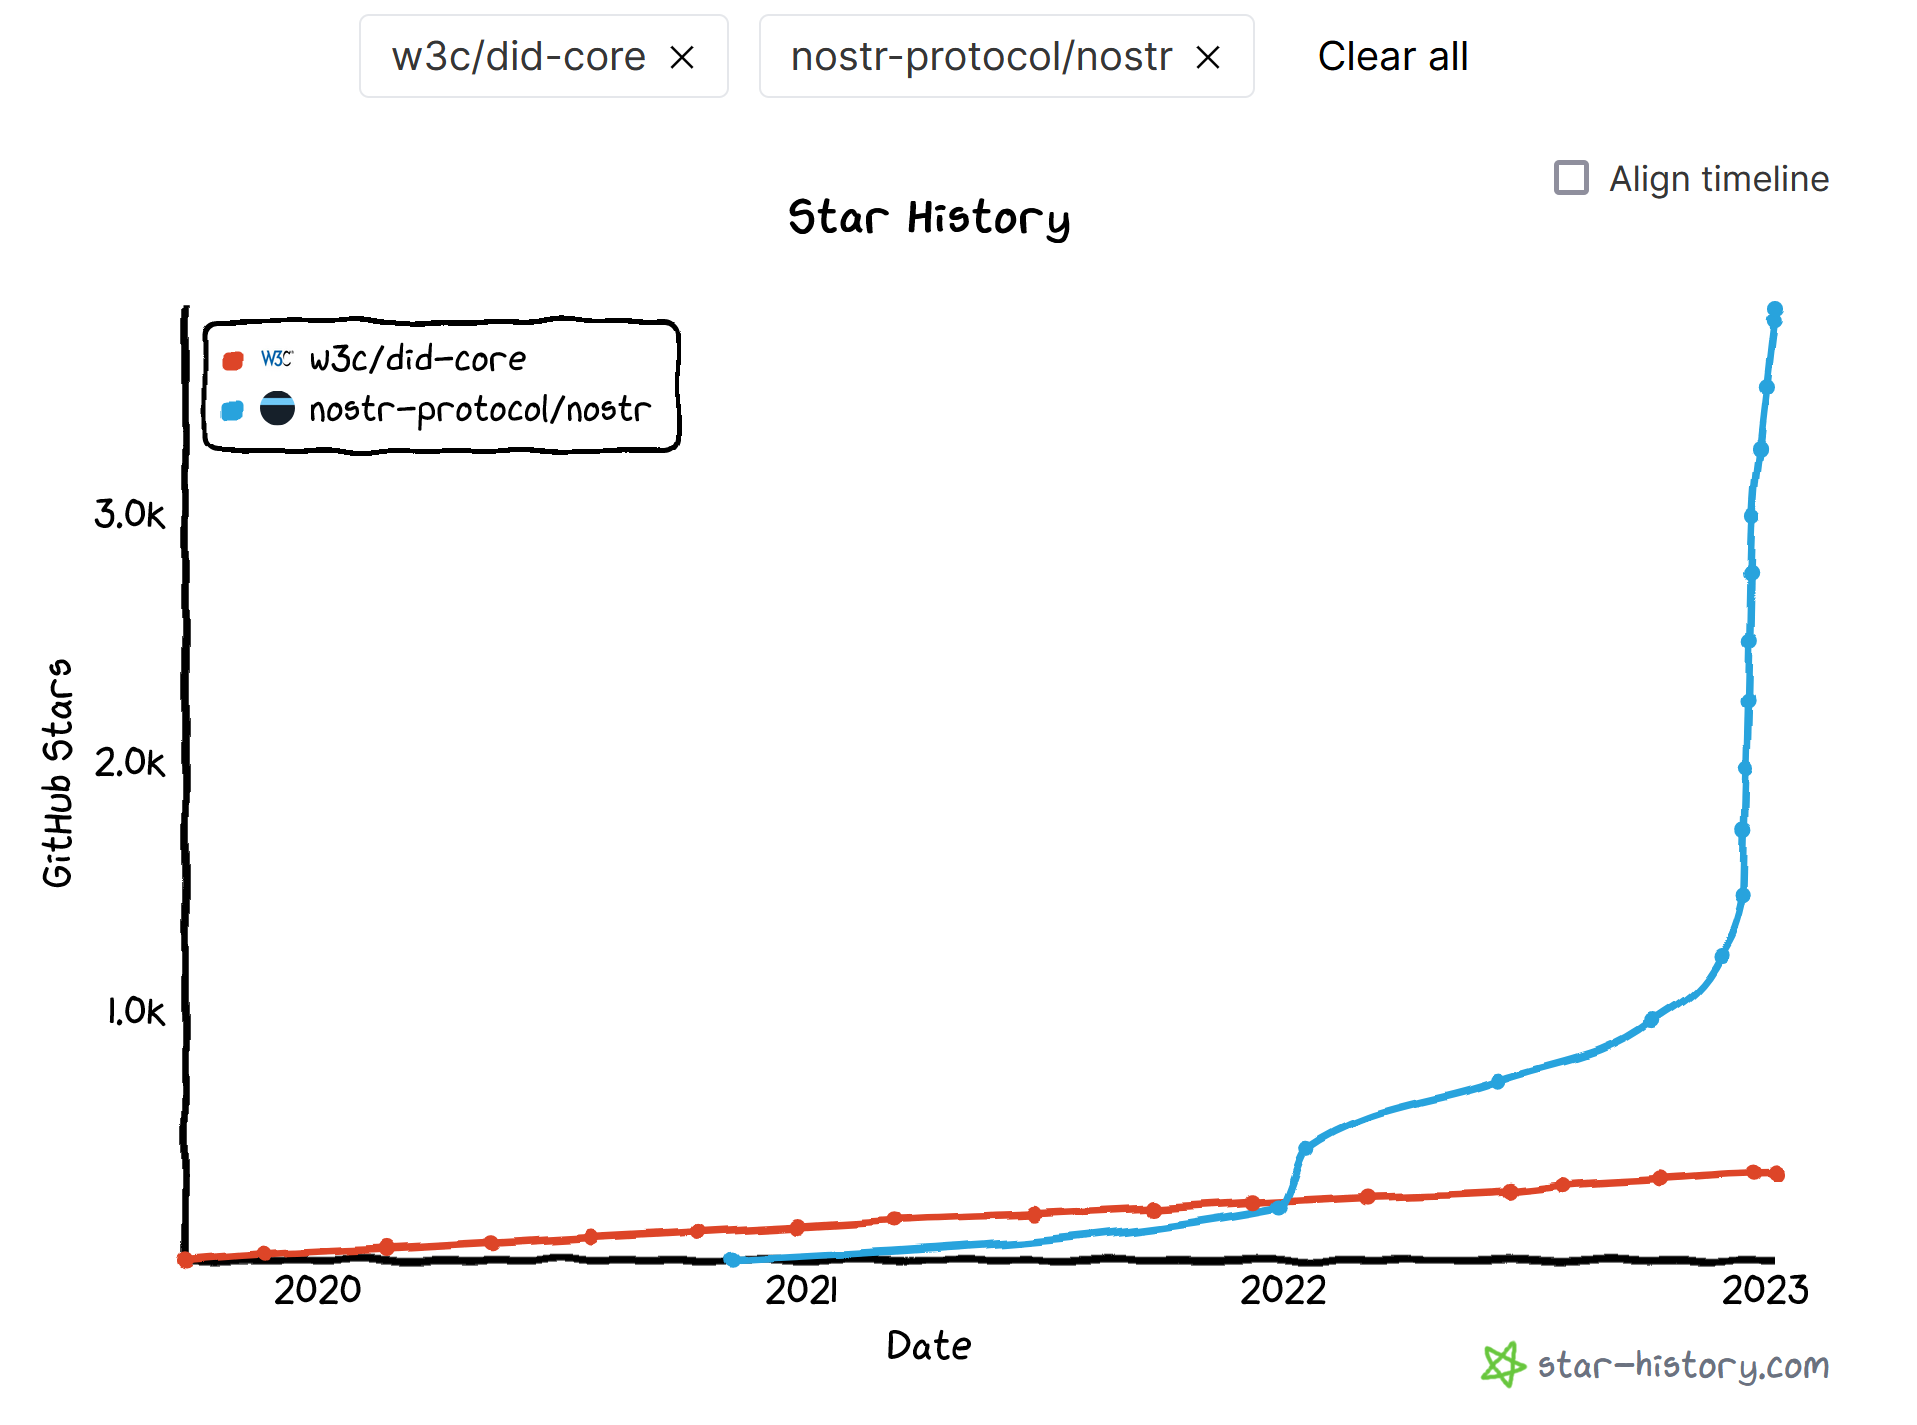
\includegraphics[width=\linewidth]{starhistory}
  \caption{An illustration of the enthusiasm for Nostr compared to traditional DID based on GitHub `stars'.}
  \label{fig:starhistory}
\end{figure}
%\subsubsection{NostrConsole}
This provides a web interface into the metaverse providing:
\begin{itemize}
\item simple cryptographic identity assurance
\item private peer to peer chat
\item group chats and channels
\item email to private message relay
\item links into media on web hosts
\end{itemize}
The pace of development on Nostr is dizzying. Peer to peer video and audio will allow us to link metaverse instances, between peers, through applications such as \href{https://monstr.app/}{Monstr}.\par
It's notable that Nostr has it's own inexpensive \href{https://github.com/lnbits/nostr-signing-device}{hardware signing device} to protect identity in situations where this might be necessary.\\
\textbf{The proposed integration of Nostr social media and messaging, a lightning layer with digital objects such as RGB, AI agents, Vircadia, and federated Bitcoin is the core value proposition of this
book.} This work pre-dates \href{https://www.theverge.com/2023/4/26/23699633/mark-zuckerberg-meta-generative-ai-chatbots-instagram-facebook-whatsapp}{Meta and Zuckerbergs} stated intent in this regard by 18 months, and is differentiated still by our focus on emerging markets and decentralisation.
\subsubsection{NIP-05}
At this time, the nascent identity layer in nostr leans on NIP-05. This is a distributed identity management system that maps Nostr keys to DNS-based internet identifiers. In events of kind 0 (setmetadata), the ``nip05'' key can have an internet identifier as its value. Clients split the identifier into the local part and domain and make a GET request to the specified URL. The response should be a JSON document with a ``names'' key containing a mapping of names to hex-formatted public keys. If the public key matches the one from the setmetadata event, the client accepts the association and considers the ``nip05'' identifier valid.\par
Clients may find users' public keys from internet identifiers by first fetching the well-known URL and then checking for a matching ``nip05''. When following public keys, clients must prioritize the keys over NIP-05 addresses. Public keys must be in hex format. Clients can enable user discovery through search boxes, allowing users to find profiles by entering internet identifiers. The identifier can be used as the ``root'' identifier, displayed as just the domain. The protocol supports both dynamic and static servers by using the local part as a query string.
\subsubsection{Nostr Protocol as the keystone}
The Nostr protocol can be used to store and share valuable content across the network. This is ably demonstrated by the \href{https://highlighter.com/}{`Highlighter' project} which allows users to store important notes from around the web using nostr. In the context of our federated social media trust model, the Nostr protocol can serve as the underlying layer that connects various instances of virtual spaces, thus enabling seamless data exchange and interoperability among them. Highlighter demonstrates that nostr events can be leveraged to create, store, and interact with valuable across networks. By utilizing this concept, we can extend the functionality to support federated social media trust, allowing users to carry their reputation, identity, and cryptographic proofs across different virtual spaces and social media platforms.
\subsubsection{Integrating Cryptographic Proofs and Reputation}
To create a trusted environment within the federated network, we must establish a mechanism for importing and verifying cryptographic proofs from various sources, such as social media sites and other digital platforms. By doing so, we enable users to bring their existing reputation and trust from these platforms into the new ecosystem, thus facilitating trust-based interactions and collaboration within the network. We can leverage the Nostr protocol and the NIP05 specification to import these cryptographic proofs, creating a secure and verifiable system for identity management and trust propagation. The NIP05 specification allows for the creation and verification of identity proofs within the Nostr protocol, thus enabling the seamless integration of trust and reputation data from external sources.\par
By utilizing the Nostr protocol as the underlying layer, we can establish connections between objects, people, and AI actors within the federated network. This interconnected ecosystem allows for seamless collaboration, information sharing, and trust-based interactions among all participants. The open-source collaboration infrastructure we propose can facilitate the development of various applications and services that leverage the federated network, such as virtual workspaces, AI-assisted creativity tools, and more. The uncensorable nature of this protocol further supports the inclusivity and accessibility we feel so important, ensuring that participants from different regions and backgrounds can take part in the digital society and contribute to its growth.\par
This federated social media trust model, built on the Nostr protocol, allows for the establishment of a robust, inclusive, and trust-based network that connects various virtual spaces, social media platforms, and AI systems. By leveraging the lessons learned from the other attempts in the space, and by maximising the inclusion of external cryptographic proofs from multiple sources, we can create a comprehensive trust system that fosters collaboration, innovation, and shared growth within the digital society.

\textbf{The proposed integration of Nostr, a lightning layer sucgh as LnBits, Vircadia, and Bitcoin is the core value proposition of this book.}\par
The Nostr protocol, with its decentralized and open-source nature, provides a solid foundation for linking and federating objects, people, and AI actors across collaborative spaces in digital society. By leveraging the Nostr protocol, we can build a robust and trust-based network that interconnects various virtual spaces, social media platforms, and AI systems. One of the key aspects of this trust-based network is the ability to import cryptographic proofs from different sources, similar to Keybase's approach to importing proofs from various social media sites \href{https://book.keybase.io/account#proofs}{(Keybase Proofs)}.
\subsubsection{CivKit}
CivKit, short for Civilization Kit, is an upcoming white paper from \href{https://www.commerceblock.com/}{Commerceblock}, discussing a decentralized and unstoppable free market solution based on Bitcoin. The project aims to build on top of Bitcoin to create an environment where anyone can trade anything with anyone else. \par
Phase one focuses on creating a marketplace built on top of Nostr, an interoperable communication protocol. This allows different services like Paxful, HODL HODL, or Nostr app to communicate and operate across each other.\par
Phase two aims to develop a mobile-friendly lightning wallet and decentralized IDs (Know Your Peer) to replace centralized KYC (Know Your Customer). This will provide a more secure and private environment for traders.\par 
CivKit is intended to be an open-source decentralized toolkit that various brands and platforms can build on top of. The goal is to facilitate peer-to-peer trading and encourage a more circular economy where people earn and spend Bitcoin rather than buying and selling it. While details are sparse it seems possible that this technology can be integrated into our systems. 

%\begin{itemize}
\item NIP-01 - basic description: The Nostr Protocol is a protocol that defines the format and flow of communication between clients and relays. It includes a structure for events, which are the only object type in the protocol, and a set of messages that clients can send to relays over a WebSocket connection. Events have a specific format and are signed using Schnorr signatures with the secp256k1 curve. Clients can send three types of messages to relays: EVENT, REQ, and CLOSE. The EVENT message is used to publish events, the REQ message is used to request events and create subscriptions, and the CLOSE message is used to stop subscriptions. The REQ message includes a subscription id and a set of filters that determine which events are sent in the subscription. Relays are expected to store the filters and send all future matching events to the same WebSocket until it is closed or replaced by a new subscription.
\item NIP-02 - contact list event type: The Nostr Protocol defines a special event with kind 3, called the "contact list", which is a list of "p" tags representing profiles that a user is following. Each tag entry includes the public key of the profile, a relay URL where events from that key can be found, and a local name or "petname" for the profile. Contact lists can be used for a variety of purposes, including backing up a list of followed profiles, discovering and displaying lists of followed profiles, sharing relay information to increase censorship resistance, and constructing local "petname" tables for easier identification of profiles. When a new contact list is published, it overwrites any previous contact lists and should be stored by relays and clients.
\item NIP-03 - open timestamp attestations: The Nostr Protocol allows for the inclusion of OpenTimestamps (OTS) attestations in events. An OTS attestation is a timestamp that serves as evidence that a document existed at a specific point in time. To include an OTS attestation in an event, it can be added to the event body under the ots key as base64-encoded OTS file data. The event's ID should be used as the raw hash to be included in the OpenTimestamps merkle tree. OTS attestations can be provided by either clients or relays, and can be used to show that an event is at least as old as the OTS date.
\item NIP-04 - encrypted direct messages: The Nostr Protocol defines a special event with kind 4, called an "encrypted direct message", which is a message that is encrypted and intended for a specific recipient. The content attribute of the event should contain the base64-encoded, AES-256-CBC encrypted message, appended by the base64-encoded initialization vector as a querystring parameter. The tags attribute should contain an entry identifying the recipient of the message using the recipient's public key. The tags attribute may also contain an entry identifying the previous message in a conversation or a message that the encrypted message is explicitly replying to, using the event ID of the previous message. The message is encrypted using a shared cipher generated by combining the recipient's public key with the sender's private key.
\item NIP-05 - DNS based identifiers: The purpose of NIP-05 is to allow users to map their public keys to internet identifiers (email-like addresses) and vice versa. This allows clients to find a user's public key by searching for their internet identifier and display that identifier instead of the public key. The process involves making a GET request to a specific URL with the user's name as a query string. The response should include a JSON object with the names and public keys of users and optional relay URLs where the user can be found. Clients should primarily reference public keys rather than internet identifiers. This is an optional feature and is not mandatory for all clients to implement.
\item NIP-06 - mnemonic seed derivation: Outlines the process for generating a public key from a mnemonic seed phrase using the BIP39 and BIP32 standards. The BIP39 standard is used to generate a mnemonic seed phrase, which is then used to generate a binary seed. The BIP32 standard is then used to derive a specific path, m/44'/1237'/0'/0/0, from the binary seed. This process is the default method for generating a public key in a single-key client. However, other types of clients may use different derivation paths for different purposes.
\item NIP-07 - browser extension spec: is a proposal for an interface that can be used by web browsers and web-based applications to interact with Nostr-based systems. The interface includes methods for getting a user's public key, signing an event, and (optionally) getting a list of relay URLs and performing NIP-04 encrypted direct messaging. The interface is intended to be used by browser extensions such as nos2x and Alby, or by the Blockcore wallet.
\item NIP-08 - mentions: specifies a method for clients to handle mentions of other events and pubkeys in the content of text note events. When a client identifies a mention, it should add the pubkey or event ID to the tags array with the tag "p" and replace the textual reference in the content with the notation "[index]", where index is the 0-based index of the related tag in the tags array. When receiving a text note event with these mentions, the client can do a search-and-replace using the actual contents from the tags array and perform any desired context augmentation.
\item NIP-09 - deletion: describes an event kind for event deletion, which includes a list of event IDs for events to be deleted. The content field of the event may contain a text note explaining the reason for the deletion. Relays should delete or stop publishing any events with the same pubkey as the deletion request, and clients should hide or indicate a deletion status for the referenced events. Relays should continue to publish deletion events indefinitely and clients should broadcast deletion events to other relays that don't have them. Clients may choose to fully hide events referenced by valid deletion events or show the event with an indication that the author has "disowned" the event. A client must validate that the pubkey of each event referenced in the deletion request is identical to the pubkey of the deletion request before hiding or deleting the event. Relays may validate this as well, but are not required to do so. There is no "undelete" functionality.
\item NIP-10 - threaded replies: This NIP describes the proper use of "e" and "p" tags in text events, which helps clients display replies in a tree structure and track the pubkeys involved in a reply thread. The "e" tag may be positional or marked with "reply" or "root" to denote the event or root of a reply chain, and the "p" tag lists the pubkeys involved in a reply thread, including the pubkey of the event being replied to.
\item NIP-11 - relay self-description: Defines the format for a Relay Information Document, which is a JSON document provided by relays to clients to inform them of their capabilities, administrative contacts, and various server attributes. The document includes a name, a description, a public key for administrative contact, an alternate contact, a list of supported NIPs, information about the software used by the relay, and a version identifier. This document is provided to clients over HTTP when they make a request with the Accept header set to application/nostr plus json to a URI that supports WebSocket upgrades.
\item NIP-12 - arbitrary tag filters: suggests the addition of a feature to allow relays (server nodes in the Nostr network) to support subscriptions to arbitrary tags in events. This feature would allow clients to search for events based on specific tags, such as location or topic. The NIP specifies that only single-letter tags can be used in queries to avoid bloating the relay indexes and to allow for easier detection of any potential abuse of the feature. The NIP provides suggestions for possible uses of this feature, including a decentralized commenting system, location-specific posts, and hashtags. However, the NIP does not standardize the use of any specific tag for any particular purpose.
\item NIP-13 - PoW: proposes the use of Proof of Work (PoW) in Nostr notes as a means of deterring spam. PoW is a computation-based proof that can be universally validated by relays and clients, and it is added to notes to provide evidence of computational work. To generate PoW for a Nostr note, a nonce tag is added to the note, and the number of leading zero bits in the note's ID is used to determine the difficulty of the PoW. Clients can use the difficulty of a note's PoW to determine whether to accept or reject it, with higher difficulty indicating a higher level of computational work. Reference code for calculating the difficulty of a note's PoW is provided in the NIP. The NIP also suggests using prefix searches to filter notes by their PoW difficulty when querying relays.
\item NIP-14 - Subject tags: proposes the use of a "subject" tag in text events, which can be used in threaded lists of messages in browsers instead of using the first few words of the message. It is similar to how email clients display lists of incoming emails by subject. When replying to a message, the subject tag should be replicated, and clients may add text to denote that it is a reply. The subject should generally be shorter than 80 characters in length.
\item NIP-15 - End of stored events: proposes a method for relays to notify clients when all stored events have been sent. The relay will send the client a "EOSE" message after it has sent all the events it has persisted, indicating that all events coming after this message are newly published. Clients should use the "supported nips" field to determine if a relay supports this feature, which is intended to reduce uncertainty and potentially simplify client code by knowing when all events have been sent.
\item NIP-16 - regular/replaceable/ephemeral event types: proposes the creation of three categories of events: regular events, replaceable events, and ephemeral events. Regular events have a kind between 1000 and 10000, and upon being received by a relay, they are sent to all clients with a matching filter and are stored. Replaceable events have a kind between 10000 and 20000, and upon being received by a relay, if they have a newer timestamp and are signed by the same key as the currently known latest replaceable event with the same kind, the old event is discarded and replaced with the newer event. Ephemeral events have a kind between 20000 and 30000, and upon being received by a relay, they are sent to all clients with a matching filter but are not stored. Clients should use the "supported nips" field to determine if a relay supports these event categories, and should not send ephemeral events to relays that do not support this NIP as they may be persisted. Replaceable events may be sent to relays that do not support this NIP, and clients querying should be prepared to receive multiple events and use the latest one. These event categories may be used in various applications such as states, typing indicators, and messaging.
\item NIP-18 - reposts: proposes the use of "reposts," which are kind 6 notes that signal to followers that another event is worth reading. The content of a repost event is empty, and it must include an "e" tag with the ID of the note being reposted, as well as a "p" tag with the pubkey of the event being reposted. The "e" tag should also include a relay URL as its third entry to indicate where it can be fetched.
\item NIP-19 - bech32/human readable encoding of keys/ids/etc: proposes the use of bech32-formatted strings to display keys, IDs, and other information in clients. These formats are not intended to be used in the core protocol, but rather for displaying to users, copy-pasting, sharing, rendering QR codes, and inputting data. It is recommended that IDs and keys be stored in hex or binary format for use in the core protocol. The NIP defines three bech32 prefixes for bare keys and IDs: "npub" for public keys, "nsec" for private keys, and "note" for note IDs. The NIP also defines two bech32 prefixes with TLV (type-length-value) contents for shareable identifiers with extra metadata: "nprofile" for nostr profiles and "nevent" for nostr events. Standardized TLV types are defined for these prefixes, including "special" for the key or ID of the profile or event, and "relay" for a relay where the entity is more likely to be found. These bech32 encodings are not intended to be used inside the standard NIP-01 event formats or filters, but are meant for human-friendly display and input. Clients should accept keys in both hex and npub format for now and convert them internally.
\item NIP-20 - event responses: proposes the introduction of "command results," which provide more information about whether an event was accepted or rejected by a relay when it is submitted. A command result is a JSON object with the structure ["OK", event id, true/false, message], where "OK" indicates that the event was either successfully saved to the database or rejected, event id is the ID of the event, true/false indicates whether the event was a duplicate and has already been saved, and message provides additional information about the success or failure of the command. Possible values for message include "duplicate," "blocked," "invalid," "pow," "rate-limited," and "error." Clients should handle these messages differently based on the prefix, such as showing error popups for "invalid" or "blocked," querying relay metadata for updated difficulty requirements for "pow," or trying again with a longer timeout for "rate-limited." Ephemeral events are not acknowledged with "OK" responses unless there is a failure. If the event or "EVENT" command is malformed and cannot be parsed, a NOTICE message should be used instead of a command result. This NIP only applies to non-malformed "EVENT" commands.
\item NIP-22 - timestamp limits: proposes a standard for relays to set limits on the timestamps of events they are willing to store. The limits would be specified as unix timestamps in seconds and would apply to all events, including regular and replaceable events. If a relay supports this NIP, it would send a command result to the client indicating whether an event was accepted or rejected due to its created at timestamp falling outside the permitted range. Clients can use the supported nips field to determine whether a relay uses event created at time limits and can handle command results accordingly. The motivation for this NIP is to improve the user experience by decreasing the number of events that appear out of order or from impossible dates in the past or future.
\item NIP-25 - reactions: A reaction is a type of note used to express a positive or negative sentiment towards another note. The content of a reaction event can be a "+" or "-", which indicates a "like" or "dislike" respectively, or an emoji. The reaction event should include the "e" and "p" tags from the note being reacted to, allowing users to be notified of reactions to their posts and enabling clients to retrieve all reactions for a specific post or thread. The "e" tag should include the ID of the note being reacted to, and the "p" tag should include the pubkey of the event being reacted to.
\item NIP-26 - delegation: describes a way for events to be signed by keypairs other than the ones that are normally used. This can be used to allow a user to generate new keypairs for each client they use, and authorize those keypairs to generate events on behalf of their root pubkey (a keypair that is stored in a secure location). The proposal introduces a new "delegation" tag that can be included in events to indicate that the event has been signed by a delegate keypair on behalf of another keypair. The proposal also describes the process for creating and using a "delegation token", which is a signature that grants authorization for the delegate keypair to sign events on behalf of the delegator.
\item NIP-28 - chat: defines new event kinds for public chat channels, messages in those channels, and basic moderation of those channels. The proposal reserves five event kinds for immediate use and five event kinds for future use. These event kinds include: creating a chat channel, setting metadata for a chat channel, sending a message in a chat channel, hiding a message in a chat channel, and muting a user in a chat channel. The proposal outlines how each of these event kinds should be used, including the data that should be included in the event and how clients and relays should handle the events.
\item NIP-33 - further replaceable events standards: adds a new range of event kinds that allow for the replacement of events that have the same "d" tag and kind. This is an extension of NIP-16, which only allowed for the replacement of events with the same kind. The proposal defines a "parameterized replaceable event" as an event with a kind of 30000 or greater, but less than 40000. The proposal outlines how these events should be handled by clients and relays, including the use of the "supported nips" field to determine support for this NIP and the use of tag filters to handle multiple events.
\item NIP-36 - Content warning: introduces the "content-warning" tag, which allows users to specify that the content of an event requires approval by readers before it is shown. The proposal describes how the tag should be used, including the optional inclusion of a "reason" for the content warning. This tag can be used by clients to hide the content of the event until the user has approved it.
\item NIP-40 - expiring events: introduces the "expiration" tag, which allows users to specify a unix timestamp at which an event should be considered expired and deleted by relays. The proposal outlines how the tag should be used, including the format of the timestamp and how it should be interpreted. The proposal also describes the behavior that clients and relays should follow when working with expired events, including the use of the "supported nips" field to determine support for this NIP and the requirement for relays to drop expired events that are published to them. The proposal suggests potential use cases for the expiration tag, including temporary announcements and limited-time offers. The proposal notes that expired events may still be accessible to third parties through the relays, and warns against using the expiration tag as a security feature.
\end{itemize}


\section{Micropayment based web}
It seems the war against disinformation is now being lost. Much is written in the media about Deepfake technology creating plausible fake videos, but probably more pernicious is the use of toolkits to create entire plausible fake news sites using natural language AI such as GPT3. This makes it cheap to publish potentially market moving news which is then rehypothecated by online news vendors who are hungry for clicks. As these pipelines become more mature it will be difficult to keep fake news for financial or political gain out of the system. One interesting way to do this that \textit{isn't} webs of trust or true cryptographic identity is to charge micropayments for ``one to many'' publication models. This would imply a tiny instant payment for clicks, especially on social media sites such as twitter. This kind of model has been discussed but is only possible in the context of systems such as Lightning where instant micropayment can be realised. It seems possible that this would price out speculative `noise' spam from the information space. It's interesting and ironic that the origin of proof of work was to underpin just such a spam defeating system  \cite{dwork1992pricing}, and that Nakamoto \href{https://www.metzdowd.com/pipermail/cryptography/2009-January/015014.html}{mentioned this application for Bitcoin} back in 2009. There is now much chatter about the integration of Bitcoin with Twitter in light of Musks buyout of the social network.
%\subsection{Open World assumption}
%\href{https://en.wikipedia.org/wiki/Open-world_assumption}{this needs unpacking}
%------------------------------------------------
%\section{File storage}
%This is a tricky section as nothing seems to work. Come back later.
%https://fiatjaf.com/d5031e5b.html
\begin{figure}
\includegraphics[width=\linewidth]{files}
  \caption{Comparison of distributed file stores}
  \label{fig:Files}
\end{figure}. 
\section{Are DAOs useful for us?}
A distributed autonomous organisation, or DAO is a governance structure which is built in distributed code on a blockchain smart contract system. Token holders have voting rights proportional to their holding. The first decentalised autonomous organisation was simply called ``The DAO'' and was launched on the Ethereum network in 2016 after raising around \$100M. \href{https://www.gemini.com/cryptopedia/the-dao-hack-makerdao#section-what-is-a-dao}{It quickly succumbed to a hack and the money was drained}. This event was an important moment in the development of Ethereum and resulted in a code fork which preserves two separate versions of the network to this day, though one is falling into obsolescence. Again, this is covered in Shin's book on the period in extreme detail, but it seems this stuff is falling into dusty history now, leaving only a somewhat tarnished and technically shaky legacy \cite{cryptopians}. \\
In practice DAOs have very few committed `stakeholders' and the same names seem to crop up across multiple projects. Some crucial community decisions within large projects only poll a couple of dozen eligible participants. Its might be that the experiment of distributed governance is failing at this stage. \par
Perhaps more interesting is the use of the DAO concept to crowd fund global projects, currently especially for the acquisition of important art or cultural items. DAOs are also emerging as a way to fund promising technology projects, though this is reminiscent of the 2017 ICO craze which ended badly and is likely to \href{https://www.cftc.gov/PressRoom/PressReleases/8590-22}{fall foul of regulations}.\par
Within the NFT and digital art space  PleaserDAO has quickly established a strong following.
``PleasrDAO is a collective of DeFi leaders, early NFT collectors and digital artists who have built a formidable yet benevolent reputation for acquiring culturally significant pieces with a charitable twist.\par
%Opensea wrangle between IPO and governance token.\par
%ConstitutionDAO, Once upon a time in Shaolin etc 
%https://harpers.org/archive/2015/01/come-with-us-if-you-want-to-live/

\subsection{Bisq DAO}
One of the better designed DAOs is \href{https://bisq.network/dao/}{Bisq DAO}. It's slightly different design trys to address the issue of overly rigid software intersecting with more intangible and fluid human governance needs. From their website:\par
\textit{``Revenue distribution and decision-making cannot be decentralized with traditional organization structures—they require legal entities, jurisdictions, bank accounts, and more—all of which are central points of failure.
The Bisq DAO replaces such legacy infrastructure with cryptographic infrastructure to handle project decision-making and revenue distribution without such central points of failure.''}

\subsection{Risks}

The most interesting thing about DAOs is that they belong more in this money chapter than they do in blockchain. As we have seen they're finding most success as loosely regulated crowd funding platforms. If a small company did find itself wishing to explore this fringe mechanism for raising capital, then we would certainly recommend keeping a global eye on evolving regulation and the onward legal exposure of the company. 
\section{Risks \& Challenges?}
Classic DID/SSI risks fragmentations. 
In all DID applications, scaling to a world where the user is managing potentially thousands of these critical cryptographic data files is daunting.
Abstracting the guts of this away to make the use simple, and only mindful of thet right level of information, turns out to be huge problem that nobody has solved
It's not clear that users want this. 
In the case of web of trust like Slashtags it's a big piece of work for the users to rate all of their digital interactions with a trust metric.


